% Tento soubor nahraďte vlastním souborem s obsahem práce.
%=========================================================================
% Autoři: Michal Bidlo, Bohuslav Křena, Jaroslav Dytrych, Petr Veigend a Adam Herout 2019

% Pro kompilaci po částech (viz projekt.tex), nutno odkomentovat a upravit
%\documentclass[../projekt.tex]{subfiles}
%\begin{document}

\chapter{Úvod}
Podpis je jednou z~nejstarších metod používanou pro ověření totožnosti, určení autorství či udělení právního souhlasu.
V~této práci půjde především o~ověření totožnosti, které spadá pod obor zvaný biometrie.
Biometrie se zabývá analýzou biologických a behaviorálních charakteristik používaných mimo jiné k~autentizaci. 
Zkoumáním pravosti podpisu a jiných textů se zabývá písmoznalectví neboli grafognózie.
U~podpisu lze analyzovat statické a dynamické parametry písma. 

Podpis je v~praxi stále nejpoužívanější způsob autentizace. 
Podaří-li se důvěryhodně podpis napodobit, bude možnost obejít bezpečnostní zabezpečení. 
To představuje velké bezpečnostní riziko a nutnost upravení dosavadních bezpečnostních metod pro autentizaci. 
Bavíme se zde spíše o~digitálním podpisu. 
Na rozdíl od podpisu na papíře digitální podpis obsahuje i dynamické charakteristiky.
Bude tedy složitější jej zfalšovat.


%TOLE JE SPIS ABSTRAKT
%Bude třeba sestavit snímací zařízení pro získaní potřebných parametrů podpisu.
%Ze statických parametrů budeme snímat tvar i tloušťku čar a celkový vzhled podpisu. 
%Z dynamických parametrů budeme snímat tlak, sklon a průběh tahů. 
%Získané data je potřeba vhodným způsobem zpracovat a provést potřebné výpočty. 
%Upravená data je poté potřeba převést do instrukcí pro mechanickou paži, která je použita k replikaci podpisu. 
%Výsledný podpis bude porovnáván s vlastnoručním podpisem. Cílem je co nejvíce se přiblížit vlastnoručnímu podpisu.

%\section{Představení tématu}
%\section{Cíle práce}

%\section{Struktura práce}

\chapter{Teoretické základy}
Pro plné pochopení problematiky je potřeba představit základy z~několika odvětví. 
V~této části budou shrnuty všechny potřebné informace. 

\section{Pojmy}
\label{sec:pojmy}
\begin{itemize}
  \item{\textbf{Biometrie} - automatizované rozpoznávání osob na základě jejich charakteristických biologických a behaviorálních rysů.} % parafráze biometrie (str. 13) / Biometric identification - parafráze (str 3)
  \item{\textbf{Biologické autentizační metody} - zkoumají biologické charakteristiky člověka, s~jimiž se narodí. Tyto charakteristiky má každý člověk unikátní a jsou neměnitelné. Patří mezi ně například otisky prstů, skeny sítnice či duhovky.}  
  \item{\textbf{Behaviorální autentizační metody} - porovnávají behaviorální charakteristiky související s~chováním člověka. Lze například porovnávat, jakým způsobem jedinec mluví nebo jak pohybuje očima.}
  \item{\textbf{Statické parametry písma} - jde o~parametry, které nezahrnují informace o~procesu psaní podpisu. Patří mezi ně například tvar a vzhled písma, umístění podpisu na stránce nebo také tloušťka čar.}
  \item{\textbf{Dynamické parametry písma} - tyto parametry se vztahují k~samotnému průběhu psaní podpisu. Například rychlost psaní, akcelerace, tlak nebo průběh tahů.}
\end{itemize}

Dále je potřeba si ujasnit tyto tři pojmy:
\begin{itemize}
  \item{\textbf{Verifikace} - potvrzení totožnosti jedince porovnáním poskytnutého vzoru s referenčními vzorem dané osoby uloženého v databázi, % |
  za kterou se vydává. Probíhá tedy principem one-to-one.}                                                                                      % |
  \item{\textbf{Identifikace} - určení identity předem neznámého jedince.                                                                       % |
  Jde tedy o přikládání poskytnutého vzoru ke všem vzorům v databázi, tedy princip one-to-many.}                                                % |
  \item{\textbf{Autentizace} - je proces, vyskytující se především u přistupových systému.                                                      % |
  Může se u ni jednat při verifikaci i identifikaci.                                                                                            % V
  Výsledkem bývá získání nějakého statusu, například získání určitých oprávnění.}                                                               % Biometrické technologie (str. 4-5) https://www.fbi.vsb.cz/export/sites/fbi/060/.content/galerie-souboru/studijni-materialy/BiometrickeTechnologie.pdf
\end{itemize}


\section{Definice podpisu a jeho charakteristiky}
Definice podpisu je z~pohledu zákona poněkud problematická. 
Podpis jako takový není v~zákoně nijak přímo definován. 
Obecně je ale bráno za podpis vlastnoruční uvedení jména a příjmení, nebo jiného jedinečného a nezaměnitelného označení. % citace? https://www.fulsoft.cz/33/komentar-zakona-89-2012-sb-obcansky-zakonik-561-uniqueidmRRWSbk196FNf8-jVUh4EtuvCojfP1Dmx8t50X_QR_yU_dtwjPItMA/

Dynamické vlastnosti poskytují více informací a umožňují lépe identifikovat neoprávněného uživatele, pokoušejícího se podpis falzifikovat.    % V
K zaznamenání těchto dynamických vlastností je avšak zapotřebí tablet a speciální aktivní pero, které při psaní ukládá relevantní parametry.  % parafráze Citace Biometrie (str 233)

Podpis patří z části ke statickým a z části k dynamickým biometrickým vlastnostem.
Pokud se uchovává pouze výsledek psaní podpisu, lze z něj extrahovat pouze statické parametry.
Pro snímání dynamických parametrů je nutné snímat podpis v průběhu jeho psaní.
Těchto parametrů je mnoho, ale pro zjednodušení se jich používá jen omezené množství.

\section{Biometrická autentizace}
Biometrie je jedním ze tří hlavních kategorií autentizace.
autentizova se můžeme pomocí toho:

\begin{itemize}
  \item{co vlastníme - identifikační doklady, karty, čipy...}   % ? | 
  \item{co známe - přihlašovací jména, hesla...}                % ? |
  \item{čím fyzicky jsme - otisky prstu, tvář, oči, podpis...}  % ? V
\end{itemize}                                                   % parafráze Biometrie a identita člověka (str 89) 
Biometrie spadá do třetí kategorie, tedy čím fyzicky jsme. 

Biometrická autentizace probíhá na základě biologických a behaviorálních charakteristik člověka\ref{sec:pojmy}. 
Obě tyto skupiny znaků jsou pro každého člověka unikátní a nezaměnitelné. To je důvodem, proč je lze využít k~autentizaci.
Existuje spousta biometrických metod pro autentizaci, kupříkladu otisk prstu, rozpoznání obličeje, sken duhovky či sítnice, nebo dokonce pomocí používání myši. 
Každá tato metoda má své výhody a nevýhody, zejména se hodnotí přesnost, cena, komfort používání, stálost a velikost vzorku. % ?
Tato práce se zaměřuje na autentizaci pomocí podpisu.

Biometrický systém je v informačních technologiích postup pro rozpoznávání vzorů lidských vlastností.       % |
Existuje spoustu různých cest, kterými lze biometrické systémy napadnout.                                   % |
V~rámci této práce se zaměříme na seznzor, jenž je první komponentu biometrického systému (obrázek níže).   % V
Tomuto senzoru budeme předkládat falešné biometriky, tedy v~našem případě falešného podpisu.                % parafráze Biometrie (str 78)

\begin{figure}[h]
  \centering
  
\includegraphics[width=0.5\textwidth]{obrazky-figures/placeholder.pdf}
  \caption{Biometrický systém - Biometrie (str. 78)}
  \label{fig:my-pdf}
\end{figure}

\newpage

\section{Parametry podpisu}
V~rámci této práce budou snímány následující parametry:
\begin{itemize}
  \item{\textbf{Celkový vzhled podpisu}}
  \item{\textbf{Pohyb pera} ze kterého bude vypočítán celkový průběh podpisu, především pak pozice pera a rychlost psaní čar.} %při psaní pomocí akcelerometru zabudovaném v MPU-6050 
  \item{\textbf{Sklon pera}} %pomocí gyroskopu, který je také součástí MPU-6050.}
  \item{\textbf{Tlak}} %pomocí čtveřice tlakových senzorů Interlink Electronics FSR® 400.}
\end{itemize}
Kombinací těchto nasnímaných parametrů by bylo možné dostatečně věrohodně napodobit původní vlastnoruční podpis. 

\section{Rozpoznávání falzifikátů}
Rozpoznání falzifikátu probíhá u statického a dynamického podpisu odlišně, následující text se bude týkat postupu, který sdílejí.

Falzifikáty jsou vyhodnoceny na základě porovnávání uloženého vzorku v~databázi s~podpisem, kterým se daný člověk pokouší autentizovat.
Výsledkem takového porovnávání je určité procento shody parametrů.
Referenční podpis je zprůměrován z~několika vzorků, aby došlo k~potlačení náhodných jevů. %  citace? zav_prace 17183 2.3
Tyto vzorky jsou poskytnuté danou osobou při registraci do systému.

\begin{figure}[h]
  \centering
  
\includegraphics[width=0.5\textwidth]{obrazky-figures/placeholder.pdf}
  \caption{Průběh autentizace}
  \label{fig:my-pdf}
\end{figure}

Obě tyto skupiny charakteristik jsou ovlivňovány jak fyzickým, tak i psychologickým stavem člověka v~době podpisu.
To znamená, že ani též osobě se nepovede dvakrát úplně totožný podpis.
Pokud jsou podpisy naprosto stejné, nejspíše půjde právě o padělek.

Porovnávací algoritmus extrahuje důležité parametry podpisu, které poté porovnává s~referenčním vzorem. 
Následně je vypočteno celkové procento shody podpisů a na jeho základě je autentizace úspěšná či nikoli.
Je přitom důležité, aby algoritmus měl určenou správnou procentuální hodnotu shody. 

Pokud by bylo procento shody špatně zvoleno, došlo by k jednomu ze dvou problémů:
\begin{itemize}
  \item{\textbf{míra falešných odmítnutí (FRR)} - neúspěšné autentizace, které by měly být úspěšné.}
  \item{\textbf{míra falešných akceptací (FAR)} - úspěšné autentizace, které by měly být neúspěšné.}
\end{itemize}

Výše zmíněné procento shody nazýváme rovnoměrná míra chybovosti (EER), ta může být nastavena právě v bodě protnutí těchto dvou křivek (viz \ref{fig:FAR_FRR}).

\begin{figure}[h]
  \centering
  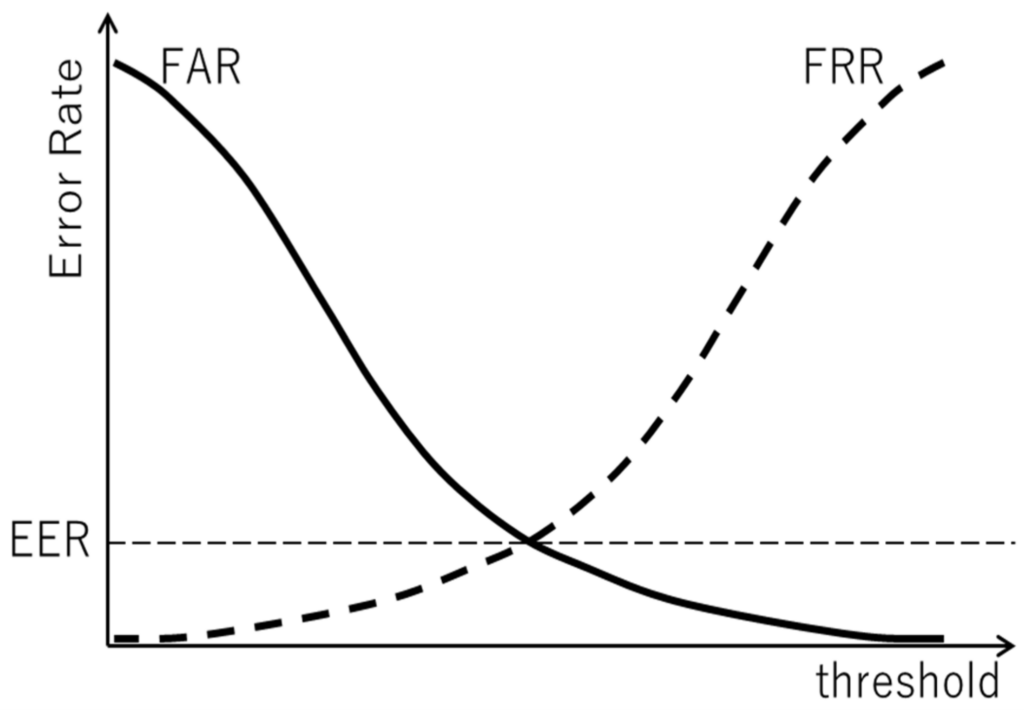
\includegraphics[width=0.5\textwidth]{obrazky-figures/FAR_FRR.png}
  \caption{Rovnoměrná míra chybovosti (EER), míra falešných odmítnutí (FAR) a míra falešných akceptací (FFR)} % https://www.cursorinsight.com/post/943/what-you-need-to-know-about-frr-and-far
  \label{fig:FAR_FRR}
\end{figure}

\newpage

\subsection{Off-line systémy pro verifikaci}
Off-line systémy pro verifikaci se rozumí systémy, které ověřují totožnost na základě statického podpisu, tedy psaného na papír.  % |
Obraz podpisu je naskenován či nasnímán kamerou a tím je získán digitální obraz podpisu.                                          % |
Tento obraz je následně porovnáván v databázi s referenčním podpisem.                                                             % |
Tato metoda je avšak nepoužitelná, co se týče automatizovaného zpracování.                                                        % V
Navíc v dnešní moderní době, při existenci skenovacích a kopírovacích zařízení, je statický podpis náchylný na falzifikaci.             % Parafráze Biografie a identita člověka (str 440)

Verifikace probíhá ve třech fázích - předzpracování, extrakce biometrických charakteristik a vyhodnocování. % |
V předzpracování projde naskenovaný obraz podpisu prahováním, vyhlazováním, normalizaci a zjednodušování.   % |
Následně jsou extrahovány biometrické charakteristiky podpisu,                                              % |
napřiklad hustota vodorovných a svislých čar, nebo vektory ohraničené oblasti.                              % |
Vyhodnocování je založeno na extrahovaných charakteristikách a jejich vektorech,                            % V
může být provedeno porovnáním významových bodů, klasifikátorem sousedů nebo neuronovou sítí.                % Parafráze Biometrie a identita člověka (strana 441 442 443) - nebo https://theses.cz/id/odwy80/BP_Vchov.pdf

\begin{figure}[h]
  \centering
  \begin{minipage}{0.3\textwidth}
      \centering
      
\includegraphics[width=\textwidth]{obrazky-figures/placeholder.pdf}
      \caption{Předzpracovaný podpis.}
      \label{fig:first-image}
  \end{minipage}\hfill
  \begin{minipage}{0.3\textwidth}
      \centering
      
\includegraphics[width=\textwidth]{obrazky-figures/placeholder.pdf}
      \caption{Extrahované parametry.}
      \label{fig:second-image}
  \end{minipage}\hfill
  \begin{minipage}{0.3\textwidth}
    \centering
    
\includegraphics[width=\textwidth]{obrazky-figures/placeholder.pdf}
    \caption{Vyhodnocování.}
    \label{fig:second-image}
  \end{minipage}
\end{figure}

\subsection{On-line systémy pro verifikaci} % preparafrazovat podle Biometrie a identita člověka str 444
On-line systémy narozdíl od off-line neporovnávají pouze výsledek podpisu, ale i data o jeho průběhu.         % |
Důležité zde jsou parametry jako změny rychlosti, tlaku a celkovém průběhu psaní podpisu.                     % |
K nasnímání těchto parametrů je potřeba tablet a speciální pero, které takové snímání umožní.                 % |
Narozdíl od statických parametrů, které lze snáze odpozorovat a napodobit,                                    % |
nebo pomocí technologií jinak replikovat, je dynamické parametry nemožné zfalšovat člověkem.                  % V
Falzifikát lze vytvořit pomocí stroje, je k tomu ale potřeba nasnímat pohyb ruky podepisujícího.              % parafráze Biometric verification (str. 170)

\begin{figure}[h]
  \centering
  \begin{minipage}{0.45\textwidth}
      \centering
      
\includegraphics[width=\textwidth]{obrazky-figures/placeholder.pdf}
      \caption{Vzhled dynamického podpisu.}
      \label{fig:first-image}
  \end{minipage}\hfill
  \begin{minipage}{0.45\textwidth}
      \centering
      
\includegraphics[width=\textwidth]{obrazky-figures/placeholder.pdf}
      \caption{Graf dynamických parametrů podpisu v~čase.}
      \label{fig:second-image}
  \end{minipage}
\end{figure}

\subsection{Biometrické normy identifikace pomocí podpisu}
Normy hrají klíčovou roli v oblasti biometrických technologií, včetně identifikace a ověřování pomocí podpisu. %!
Zajišťují jednotný přístup k ukládání, zpracování a výměně dat, což umožňuje interoperabilitu mezi různými systémy a zařízeními. %!
Díky normám je možné implementovat technologie, které splňují požadavky na bezpečnost, spolehlivost a přesnost, a zároveň odpovídají právním a regulačním standardům. %! 
V oblasti biometrického podpisu se normy zaměřují na standardizaci datových formátů, aby byla zajištěna kompatibilita mezi různými aplikacemi, jako jsou smart karty, elektronické podpisy nebo systémy pro biometrickou verifikaci. %!

Pro oblast biometrického podpisu byly vytvořeny následující klíčové normy: %!

\begin{itemize}
  \item{\textbf{ISO/IEC 19794-7:2007}: Tato norma specifikuje dva formáty pro výměnu dat o podpisu a písmu. První je obecný formát určený pro široké použití, zatímco druhý, kompaktní formát, je optimalizován pro použití na zařízeních s omezenými zdroji, jako jsou smart karty. (Zdroj: ISO 19794-7:2007)} %!
  \item{\textbf{ISO/IEC 19794-11:2013}: Norma popisuje obecný formát výměny dat pro zpracované dynamické údaje o podpisu či písmu. Tyto údaje jsou získávány z časových řad zachycených specializovanými zařízeními, a slouží k biometrickému porovnání. (Zdroj: ISO 19794-11:2013)}%!
  \item{\textbf{ANSI/INCITS 395-2005}: Tato norma se zaměřuje na formát výměny dat pro digitalizované písmo a podpis. Jejím cílem je podpora biometrického zápisu, verifikace nebo identifikace. Tento obecný formát je využitelný v širokém spektru aplikací, které pracují s elektronickými podpisy. (Zdroj: ANSI/INCITS 395-2005)}%!
\end{itemize}

Normy jako ISO/IEC 19794 a ANSI/INCITS 395-2005 přinášejí několik zásadních výhod:%!
\begin{itemize}
    \item{Interoperabilita: Umožňují výměnu dat mezi různými systémy a zařízeními bez ztráty integrity nebo kompatibility.}%!
    \item{Bezpečnost: Standardizované formáty zajišťují ochranu citlivých dat a minimalizují riziko neoprávněného přístupu.}%!
    \item{Spolehlivost: Poskytují jednotné metody pro ukládání a zpracování dat, což zvyšuje přesnost a důvěryhodnost biometrických systémů.}%!
    \item{Právní jistota: Splnění norem často znamená, že technologie odpovídá požadavkům právních a regulačních předpisů, což je klíčové pro jejich nasazení v komerčním nebo veřejném sektoru.}%!
\end{itemize}

Normy v oblasti biometrického podpisu tedy představují základní stavební kámen pro efektivní a bezpečné nasazení těchto technologií v praxi.%!

\chapter{Analýza současných řešení}
Technologie automatického ověřování podpisu se v současnosti řadí mezi klíčové oblasti výzkumu.                                                         % |
Především díky své důležitosti ve vědeckém a komerčním kontextu.                                                                                        % |
S rychlým rozvojem internetu a rostoucími požadavky na bezpečnost v digitální společnosti se tato technologie stává stále relevantnější.                % |
Poskytuje efektivní a důvěryhodnou metodu ověřování identity, která je v současnosti široce akceptována jak z právního, tak ze společenského hlediska.  % V
To ji činí zásadním nástrojem pro současné technologické aplikace.                                                                                      % Impedovo

\section{Současná řešení v~oblasti biometrie}
Nedávné mezinárodní soutěže využívající standardní databáze a testovací protokoly přinesly zajímavé výsledky.   % |
Ukázalo se, že systémy pro ověřování podpisů dosahují vysoké přesnosti.                                         % V
Tato úroveň přesnosti je srovnatelná s jinými pokročilými biometrickými technologiemi.                          % C. Vielhauer, “A behavioural biometrics,” Public Service Rev.: Eur.Union, vol. 20, no. 9, pp. 113–115, 2005.

Na rozdíl od fyziologické biometrie je vlastnoruční podpis aktivní metodou.                                                   % |
Ta vyžaduje, aby uživatel provedl konkrétní akci podpisu.                                                                     % V
Automatické ověřování podpisu je tedy obzvláště užitečné v aplikacích, kde je nutná autentizace jak uživatele, tak transakce. % Plamondon and S. N. Srihari, “On-line and offline handwriting recog-nition: A comprehensive survey,” IEEE Trans. Pattern Anal. Mach.Intell., vol. 22, no. 1, pp. 63–84, Jan. 2000

Systémy pro verifikaci podpisu se obvykle skládají z hardwarových a softwarových komponent.%!
Ty spolupracují při ověřování autenticity podpisu. %!
Zařízení pro sběr podpisu mohou zahrnovat dotykové obrazovky, grafické tablety nebo speciální senzory, zaznamenávající různé parametry podpisu.%!
Takovými parametry jako je tlak, rychlost a trajektorie pohybu ruky. % \cite{novak2022}, \cite{kriz2019}.%!

\section{Systém, zařízení a kde se využívají, a jak jsou důvěryhodné}
Tyto systémy jsou široce využívány v bankovnictví, právních službách, elektronických platbách a dalších oblastech, ve kterých je nutné ověřit identitu uživatele a zajistit integritu transakce.%!
Důvěryhodnost těchto systémů závisí na několika faktorech, včetně kvality zařízení pro sběr dat, algoritmů pro analýzu podpisu a úrovně šifrování použité při přenosu dat. %!
Vysoká úroveň přesnosti a spolehlivosti je kladně ovlivněna používáním pokročilých metod strojového učení a biometrických analýz, které zajišťují, že systém dokáže rozlišit mezi autentickým podpisem a padělaným. %!
Přesto i u těchto systémů existují určité výzvy, jako je možnost podvodů prostřednictvím simulace podpisu nebo použití záznamů starých podpisů. %!
Z tohoto důvodu je důležité kombinovat různé metody autentizace pro dosažení co nejvyšší úrovně bezpečnosti. % \cite{vodicka2021}, \cite{hanzelka2020}.%!

\section{Hodnocení výhod a nevýhod existujících řešení}
Existující řešení pro verifikaci podpisu nabízejí několik výhod a nevýhod v závislosti na použité technologii a aplikacích. %!
Mezi hlavní výhody patří vysoká úroveň bezpečnosti, kterou poskytují biometrické metody.%!
Analýza dynamiky podpisu, jako je měření rychlosti, tlaku a trajektorie pohybu ruky, zvyšuje spolehlivost ověření podpisu a umožňuje detekci padělaných podpisů, což je klíčové pro oblasti, jako je bankovnictví a právní služby. % \cite{Jain2004}, \cite{Kumar2016} %!
Systémy pro verifikaci podpisu mohou být rovněž snadno implementovány v digitálních prostředích, což usnadňuje autentizaci uživatelů při online transakcích a zajišťuje integritu dokumentů.%!

Na druhé straně existují i nevýhody, které je třeba zvážit při implementaci těchto systémů. %!
Jedním z hlavních problémů je vysoká cena potřebného hardwaru a softwaru, což může být pro některé organizace překážkou. %!
Další výzvou je náchylnost biometrických systémů k podvodům, jako je použití padělaných podpisů nebo záznamů starých podpisů, což může ohrozit bezpečnost. % \cite{Kose2017} %!
Kromě toho přesnost systémů pro verifikaci podpisu může být ovlivněna faktory, jako jsou změny v rukopisných schopnostech uživatele, což může vést k falešným odmítnutím nebo akceptacím podpisu. %\cite{Rathgeb2016}. %!
Tyto faktory ukazují, že biometrické systémy nejsou bez rizika a měly by být kombinovány s dalšími metodami autentizace pro zajištění maximální bezpečnosti.%!

Závěrem lze říci, že existující řešení pro verifikaci podpisu nabízejí vysokou úroveň bezpečnosti a efektivity, ale také čelí výzvám, které vyžadují pečlivé zvážení při jejich implementaci a použití.%!

\section{Výběr senzorů a technologií}
Výběr senzorů pro nasnímání dynamických parametrů byl složitý vzhledem k rozměru pera a omezenému rozpočtu. % |
Dalším parametrem, který hrál roli při rozhodování, byla přesnost jednotlivých komponent.                   % V
Bylo důležité brát v potaz i to, zda jsou všechny komponenty kompatibilní s použitým mikrořadičem.          % vlatní kec

\subsection*{ESP32}
Mikrořaďič ESP32 je jedním z nejrozšířenějších mikrořadičů používaných ve světě.                            % |
V tomto projektu je osazen na vývojové desce ESP32 DevKitC od firmy Espressif.                              % V
Ta je jednou z nejpopulárnějších vývojových desek založených na mikrořadiči ESP32.                          % The Official ESP32 book (str. 35)
Vývojová deska ESP32 DevKitC zde slouží jako mozek celého snímání.                                          % |
Jsou k ní připojené všechny ostatní komponenty, které právě mikrořadiči odesílají nasnímaná data.           % V
ESP32 poté tyto data zpracovává a odesílá je do počítače, ke kterému je připojen  pomocí USB kabelu.        % vlastní kec

\subsection*{MPU-6050 (akcelerometr a gyroskop)}
MPU-60X0 je první integrované zařízení na světě pro sledování pohybu v šesti osách pomocí           % |
kombinace tříosého gyroskopu, tříosého akcelerometru a digitálního procesoru pohybu.                % V
Je široce využívaný v mnoha odvětvích, kde je potřeba schopnosti přesně sledovat pohyby uživatele.  % https://invensense.tdk.com/wp-content/uploads/2015/02/MPU-6000-Datasheet1.pdf

Zde slouží ke stejnému účelu, a to snímaní dat pohybu pera při podpisu.                             % |
Jak bylo zmíněno v kapitole XY, tyto data jsou potřebná pro extrakci dynamických parametrů podpisu. % V
Snímaná data jsou odesílána v reálném čase mikrořadiči ESP32.                                       % vlastní kec

\subsection*{Tlakový senzor Interlink Electronics FSR® 400}
Model FSR 400 je jednozónový tlakový senzor, tedy má pouze jednu aktivní měřící plochu.                       % |
Rezistory FSR jsou dvouvodičová zařízení a používají robustní polymerové tlustovrstvé snímače.                % |
Ty s rostoucím tlakem na snímač snižují odpor, lze tedy pomocí protékajícího proudu vypočítat sílu stlačení.  % V
Minimální aktivační síla je 0,1 N a maximální citlivost je do 20 N.                                           % https://www.interlinkelectronics.com/fsr-400


\chapter{Návrh snímacího pera}
Pro nasnímání podpisu bylo potřeba sestrojit speciální pero.                                        % |
Toto pero v průběhu podepisování zaznamenává polohu pera ve trojrozměrném prostoru,                 % |
jeho náklon a tlak, který je perem vyvíjen na papír.                                                % |
V rámci této práce není důležité, aby tyto snímače a celkový systém byl skrytý před uživatelem.     % |
Šlo tedy pouze o vymodelování pera, do kterého bude možné jednotlivé komponenty uložit.             % |
Komponenty bylo nutné připevnit pevně, aby bylo možné snímat přesné a korektní informace o podpisu. % |
Pokud by jednotlivé komponenty nebyly správně upevněny,                                             % V
mělo by to negativní vliv na nasbírané informace a tedy na celou replikaci podpisu.                 % vlastní kec
 
\section{Schéma a popis návrhu}



\section{Možnosti replikace podpisu}

%\chapter{Implementace prototypu}
%\section{Vývoj hardwaru}
%\section{Sbírání dat v~reálném čase}
%\section{Ukládání dat pro následnou replikaci podpisu}

%\chapter{Replikace podpisu}
%\section{Využití robotické ruky}
%\section{Transformace nasnímaných dat na kód pro replikaci}
%\section{Testování a výsledky replikace}

%\chapter{Hodnocení výsledků}
%\section{Analýza dosažených výsledků}
%\section{Porovnání s~očekáváními}
%\section{Diskuze o~spolehlivosti a přesnosti replikace}

%\chapter{Závěr}
%\section{Shrnutí hlavních poznatků}
%\section{Zhodnocení významu práce}
%\section{Budoucí perspektivy}

%\section{Možná vylepšení a rozšíření}
%\*subsection{Návrhy na zlepšení prototypu}
%\*subsection{Možnosti dalšího výzkumu a vývoje}


%===============================================================================

% Pro kompilaci po částech (viz projekt.tex) nutno odkomentovat
%\end{document}
